\documentclass[11pt, oneside]{article}   	% use "amsart" instead of "article" for AMSLaTeX format
\usepackage{geometry}                		% See geometry.pdf to learn the layout options. There are lots.
\geometry{letterpaper}                   		% ... or a4paper or a5paper or ... 
%\geometry{landscape}                		% Activate for for rotated page geometry
%\usepackage[parfill]{parskip}    		% Activate to begin paragraphs with an empty line rather than an indent
\usepackage{graphicx}				% Use pdf, png, jpg, or eps� with pdflatex; use eps in DVI mode
								% TeX will automatically convert eps --> pdf in pdflatex		
\usepackage{amssymb}
\usepackage{amsmath}
\usepackage{parskip}
\usepackage{color}
\usepackage{hyperref}

\title{Orthogonality of sine and cosine:  using exp}
%\author{The Author}
%\section{}
%\subsection*{}
\date{}							% Activate to display a given date or no date

\graphicspath{{/Users/telliott_admin/Dropbox/Tex/png/}}
% \begin{center} 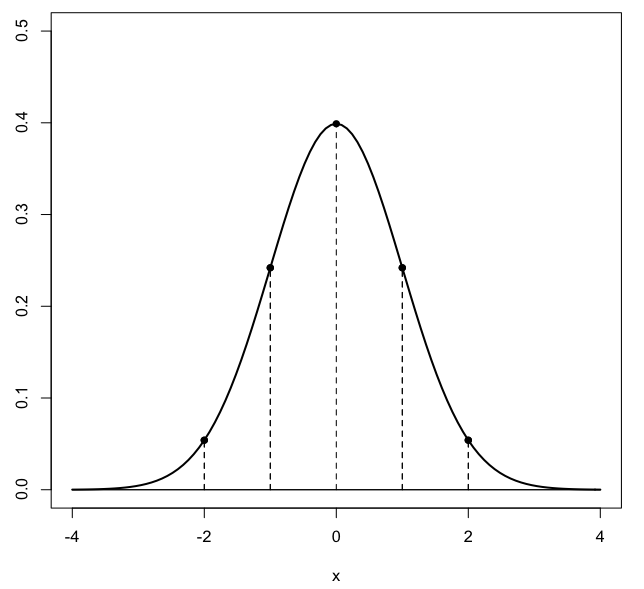
\includegraphics [scale=0.4] {gauss3.png} \end{center}
\begin{document}
\maketitle
\Large
I want to take another look at the basic identities that are used in building up Fourier series.  We're interested in products of sine and cosine like
\[ \cos nx \ \cos mx \]
\[ \sin nx \ \sin mx \]
\[ \sin nx \ \cos mx \]
There may be other factors as well
\[ \cos \frac{n\pi}{L}x \ \cos \frac{n\pi}{L} mx \]
but I'm going to treat the simple case here.  The result we had before was that (over an appropriate interval which is a multiple of $\pi$), such products are always $0$ if $m \ne n$, whereas if $m=n$ then the integrals are very simple, but do depend on whether $m=n=0$ or $m=n\ne 0$.
\section*{$\cos nx \ \cos mx$}
This one is more easily treated with the trig approach.  Let's see
\[ \cos s + t = \cos s \cos t - \sin s \sin t \]
\[ \cos s - t = \cos s \cos t + \sin s \sin t \]
Adding them together
\[ \cos s + t + \cos s - t = 2 \cos s \cos t \]
So
\[ \cos nx \ \cos mx = \frac{1}{2} \ [ \ \cos (n+m)x + \cos(n-m)x \ ] \]
When integrated over an interval like
\[ \int_{-\pi}^{\pi} \cos nx \ \cos mx \ dx  = \frac{1}{2} \int_{-\pi}^{\pi} \cos (n+m)x + \cos(n-m)x \ dx \]
\[ = \frac{1}{2} \ [ \ \frac{\sin(n+m)x}{n+m} + \frac{\sin(n-m)x}{n-m} \ ] \ \bigg |_{-\pi}^{\pi} \]
if $n\ne m$ then since $n$ and $m$ are integers both terms on the right side are equal to zero, since $\sin k \pi = 0$ for integer $k$, including $k=0$.

However, if $n=m$ then there are two cases.  If $n=m\ne 0$ the left-hand term is zero as we just saw.  Looking at the integrated form, it seems we have a problem, since we're attempting to divide by zero, luckily the right-hand term in the integral above it is $\int \cos(0) \ dx = \int dx$ which is just $x$, which gives us $2 \pi$ times one-half, which is $\pi$.

If $m=n=0$, then we have double this value.  Let's apply this logic to the more complicated argument and limits used by Paul
\[ \int_{-L}^{L} \cos \frac{n\pi x}{L} \cos \frac{m \pi x}{L} \ dx \]
\[ = \frac{1}{2} \ [ \ \int_{-L}^{L} \cos \frac{(n+m)\pi x}{L} + \cos \frac{(n-m)\pi x}{L} \ dx \ ]  \]
For integer $n$ and $m$, the left-hand term is
\[ \cos (n+m)\pi - \cos -(n+m) \pi \]
\[ = \cos (n+m)\pi - \cos (n+m) \pi = 0 \]
and the right is the same.  Otherwise, we have either one or two terms of $L$ (remembering the factor of one-half from outside the integral).

If we were to do this with exponentials, it is arguably more complicated
\[ \cos nx = \frac{1}{2} (e^{inx} + e^{-inx}) \]
\[ \cos nx \cos mx = \frac{1}{4} (e^{inx} + e^{-inx})(e^{imx} + e^{-imx}) \]
\[ = \frac{1}{4}(e^{i(m+n)x} + e^{i(n-m)x)} + (e^{-i(n-m)x} + e^{-i(n+m)x}) \]
\[ = \frac{1}{2}(\frac{e^{i(m+n)x} + e^{-i(n+m)x}}{2} + \frac{e^{i(n-m)x} + e^{-i(n-m)x}}{2} ) \]
\[ = \frac{1}{2} \ [ \ \cos (n+m)x + \cos(n-m)x \ ] \]
which is just what we had.

I'm not going to do the sine times sine.  But let's look at
\[ \sin nx \ \cos mx \]
\[ = \frac{1}{4i}(e^{inx} - e^{-inx})(e^{imx} + e^{-imx}) \]
\[ = \frac{1}{4i}(e^{i(m+n)x} + e^{i(n-m)x} - e^{i(m-n)x} - e^{-i(m+n)x}) \]
\[ = \frac{1}{4i}(e^{i(m+n)x} + e^{i(n-m)x} - e^{-i(n-m)x} - e^{-i(m+n)x}) \]
\[ = \frac{1}{4i}(e^{i(m+n)x} - e^{-i(m+n)x}) \]
\[ = \frac{1}{2}(\sin (m+n) x ) \]
so
\[ \int_{-\pi}^{\pi} \sin nx \ \cos mx \ dx = \frac{1}{2} \int_{-\pi}^{\pi} \sin (m+n) x \ dx = 0 \]
since $\sin k \pi = 0$ for integer $k$, including $k=0$.

\end{document}  